\chapter{Rekursive Datentypen und Strukturelle Rekursion}
\section{Listen}
Mit Strukturen können Datenobjekte mit einer festen Zahl von Daten gespeichert werden. Häufig wissen wir jedoch nicht, aus wie vielen Datenelementen eine Datenstruktur besteht.
%%%%%%%%%%%%%%%%%%%%%%%%%%%%%%%%%%%%%%%%%%%
Oder die Struktur der Daten ist rekursiv.
%???? KEINE AHNUNG WAS MIT DEM LETZTEN SATZ GEMEINT IST!!!
Mit rekursiven Datentypen können auch beliebig große Datenobjekte strukturiert abgespeichert werden. Die Idee davon ist die Folgende: Ein Element der Datenstruktur speichert (direkt oder indirekt) ein Exemplar der Datenstruktur. Dies nennt man dann eine \textit{rekursive Datenstruktur}. Um eine \uline{endliche} Datenstruktur zu bekommen benötigt man einen \textit{Rekursionsanker}. Diesen Rekursionsanker modellieren wir mit der Technik zu heterogenen Daten aus dem letzten Kapitel.

Eine Liste ist entweder die leere Liste \textit{the-emtpylst}, oder \textit{(make-lst s r)}, wobei s ein Wert ist und r eine Liste. Im folgenden sehen wir eine Modellierung von Listen mit Struktur.

\begin{lstlisting}{t03-prog1}
;; a list with 0 elements
;; (define list0 the-emptylst)
(define list0 empty)

;; a list with 1 element
;; (define list1 (make-lst 'a the-emptylst))
(define list1 (cons 'a empty))

;; a list with 2 elements
;; (define list2 (make-lst 'a
;;               (make-lst 'b the-emptylst)))
(define list2 (cons 'a (cons 'b empty)))

;; get the 2nd element from list2
;; (lst-first (lst-rest list2)) -> 'b
(first (rest list2)) ;; -> 'b
\end{lstlisting}

Listen sind ein wichtiger Datentyp, weshalb es einen eingebauten Datentyp existiert. Der Konstruktor \textit{cons} besitzt zwei argumente. cons entspricht unserem \textit{make-lst} Eigenbeispiel und steht wie es leicht zu vermuten ist für \textit{cons}truktor. Zudem existiert eine leere Liste \textit{emtpy} die unserer leeren Liste \textit{the-emptylst} entspricht. Auf die Sektoren der Liste kann man mit \textit{first} und \textit{rest} zugreifen. Mit \textit greift man auf das erste Element und mit \textit{rest} auf den Rest der Liste zu. Zudem haben beide noch \textit{historische Namen} die da lauten \textit{car} für \textit{first} und \textit{cdr} für rest. Die Prädikate \textit{lst?} und \textit{emtpy?} entsprechen \textit{lst?} und \textit{emptylst?}.
\textit{lst?} checkt ob es eine Liste ist und \textit{emptylst?} ob die Liste leer ist. Im Folgenden nun ein Beispiel:


\begin{lstlisting}{t03-prog2}
; a list with 0 elements
;; (define list0 the-emptylst)
(define list0 empty)

;; a list with 1 element
;; (define list1 (make-lst 'a the-emptylst))
(define list1 (cons 'a empty))

;; a list with 2 elements
;; (define list2 (make-lst 'a
;;               (make-lst 'b the-emptylst)))
(define list2 (cons 'a (cons 'b empty)))

;; get the 2nd element from list2
;; (lst-first (lst-rest list2)) -> 'b
(first (rest list2)) ;; -> 'b
\end{lstlisting}

Wie sie sehen besteht der einzige Unterschied zwischen \textit{make-lst} und \textit{cons} darin, dass \textit{cons} als zweites argument \textit{empty} oder \textit{(cons ...)}. Zum Beispiel :

\begin{lstlisting}{t03-prog3}
(cons 1 2)
\end{lstlisting}
ist ein Fehler
\begin{lstlisting}{t03-prog3}
(make-lst 1 2)
\end{lstlisting}
aber nicht.\\
\textit{cons} verhindert also inkorrekte Nutzung der Prozedur. In anderen LISP-basierten Dialekten fehlt allerdings diese Überprüfung. \\\\
Eine bessere Emulation sähe wie folgt aus:

\begin{lstlisting}{t01-prog4}
(define-struct lst (first rest))
(define-struct emptylst ())
(define the-emptylst (make-emptylst))
(define (our-cons a-value a-list)
  (cond
    [(emptylst? a-list) (make-lst a-value a-list)]
    [(lst? a-list) (make-lst a-value a-list)]
    [else (error 'our-cons "list as second argument expected")]))
\end{lstlisting}
Dies kann aber nicht verhindern, dass man \textit{make-lst} direkt verwendet. Im folgenden noch einige visuelle Beispiele.

\begin{lstlisting}{t03-prog4}
(cons 'Mercury empty)
\end{lstlisting}
\\
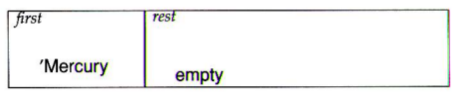
\includegraphics[height=2cm]{Bilder/T03_00.png}

\begin{lstlisting}{t03-prog4}
(cons 'Venus
    (cons 'Mercury empty))
\end{lstlisting}
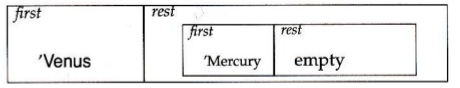
\includegraphics[height=2cm]{Bilder/T03_01.png}

\begin{lstlisting}
(cons 'Earth
  (cons 'Venus
	  (cons 'Mercury empty)))
\end{lstlisting}
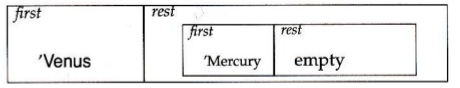
\includegraphics[height=2cm]{Bilder/T03_01.png}

In den folgenden Beispielen sehen wir: Listen speichern beliebige Datentypen, auch gemischte Daten.

\begin{lstlisting}{t03-prog5}
(cons 0
  (cons 1
    (cons 2
      (cons 3
        (cons 4
      	  (cons 5
            (cons 6
              (cons 7
                (cons 8
                  (cons 9 empty))))))))))
\end{lstlisting}

\begin{lstlisting}{t03-prog6}
(cons 'RobbyRound
  (cons 3
    (cons true empty)))
\end{lstlisting}
\section{Abgeschlossenheitseigenschaft}
Eine Operation zum Kombinieren von Daten besitzt die Abgeschlossenheitseigenschaft, wenn die Ergebnisse der Kombination von Datenobjekten wiederum mit der Operation kombiniert werden können.  \textit{cons} ist hier ein gutes Beispiel. Solche Kombinationsoperatoren können verwendet werden, um hierarchische Daten aufzubauen. \\\
Doch sind wir der Abgeschlossenheit schon einmal begegnet?\\
Der Ursprung des Begriffs „Abgeschlossenheit“ (engl. closure) kommt aus der abstrakten Algebra. Es gilt:
\begin{quote}
	Eine Menge von Elementen ist abgeschlossen bezüglich einer Operation, wenn die Anwendung der Operation an Elementen der Menge wieder ein Element der Menge produziert.
\end{quote}
Der Gedanke, dass ein Mittel der Kombination die Abgeschlossenheitseigenschaft besitzen soll, ist intuitiv, jedoch erfüllen Kombinationsoperatoren vieler Programmiersprachen diese nicht. So kann man Elemente kombinieren, indem man diese in Arrays (->T11.84ff) speichert. Man kann aber unter Umständen keine Arrays aus Arrays zusammenstellen bzw. als Rückgabewerte von Prozeduren verwenden. Es fehlt ein eingebauter „Universalkleber“, der es einfacher macht, zusammengesetzte Daten in einer uniformen Art und Weise zu manipulieren.

\subsection{list Konstruktor}
Längere Listen mit \textit{cons} zu erzeugen ist unhandlich, daher gibt es in den HtDP-TL den Konstruktor \textit{list}. Dieser bekommt eine beliebige Menge von Argumenten und erzeugt eine Liste mit allen Argumenten als Elementen. Als Beispiel:

\begin{lstlisting}{t03-prog7}
(list 1 2 3)
\end{lstlisting}
statt
\begin{lstlisting}{t03-prog7}
(cons 1 (cons 2 (cons 3 empty)))
\end{lstlisting}
oder zum Beispiel:
\begin{lstlisting}{t03-prog8}
(list (list 'a 1) (list 'b 2))
\end{lstlisting}

Allgemein gilt
\begin{lstlisting}{t03-prog9}
(list exp-1 ... exp-n)
\end{lstlisting}
 äquivalent zu
\begin{lstlisting}{t03-prog9}
(cons exp-1 (cons ... (cons exp-n empty))...)
\end{lstlisting}

\subsection{Der ' oder quote Konstruktor}
Da Listen wirklich sehr oft eingesetzt werden können einige Listen können mit Hilfe des Quote-Konstruktors ' noch weiter abgekürzt werden.
\begin{lstlisting}{t03-prog10}
'(1 2 3)
\end{lstlisting}
ist die Kurzform für
\begin{lstlisting}{t03-prog10}
(list 1 2 3)
\end{lstlisting}
\\
Ein weiteres Beispiel:
\begin{lstlisting}{t03-prog11}
'((1 2) (3 4) (5 6))
\end{lstlisting}
steht für
\begin{lstlisting}{t03-prog11}
(list (list 1 2) (list 3 4) (list 5 6))
\end{lstlisting}
dies sollte man nicht verwechseln mit (list a b c) – list wertet alle
Argumente aus, quote jedoch nicht. \\Im Allgemeinen bedeutet also
\begin{lstlisting}{t03-prog12}
'(e-1 ... e-n)
\end{lstlisting}
steht für
\begin{lstlisting}{t03-prog12}
(list 'e-1 ... 'e-n)
\end{lstlisting}
Achtung:\\
\textit{'exp-i} ist ein Symbol, wie z.B. \textit{'+'}, \textit{'true}, \textit{'list (!!!)}. Nur für Zahlen gilt \textit{'e-i = e-i}. Beachten Sie, dass diese Regel rekursiv ist! Um list und quote zu verwenden, stellen Sie ab jetzt DrRacket um auf den Sprachlevel “Beginning Student with List Abbreviations” bzw. „Anfänger mit Listen-Abkürzungen“!

\subsection{Verarbeitung rekursiver Datentypen}
Jetzt kann man sich die Frage stellen wie wir nun unsere Exemplaren rekursiven Datentypen? Die Antwort ist simpel: Wir benutzen unser Designrezept für heterogene Daten.\\

1. Schritt: Definition des Vertrags, Header etc. \\
Beachten Sie die Konvention (listof XXX), um im Vertrag zu dokumentieren, \\
was für Daten als Listenelemente erwartet werden.
\begin{lstlisting}{t03-prog13}
;; contains-doll?: (listof symbol) -> boolean
;; to determine whether the symbol 'doll occurs
;; in a-list-of-symbols
(define (contains-doll? a-list-of-symbols) ...)
\end{lstlisting}

2. Schritt: Tabelle erstellen:\\
Für jeden Datentyp ein cond-Zweig u. Selektoren andeuten\\
\begin{lstlisting}[firstnumber=4]
(define (contains-doll? a-list-of-symbols)
  (cond
    [(empty? a-list-of-symbols) ...]
    [(cons? a-list-of-symbols)
        ... (first a-list-of-symbols) ...
        ... (rest a-list-of-symbols) ...]))
\end{lstlisting}\\
Der Erster Fall (leere Liste) ist trivial
\begin{lstlisting}[firstnumber=6]
[(empty? a-list-of-symbols) false]
\end{lstlisting}

Mit den verfügbaren Daten können wir direkt das erste Element
der Liste überprüfen.

\begin{lstlisting}[firstnumber=7]
[(cons? a-list-of-symbols)
  (cond
    [(symbol=? (first a-list-of-symbols) 'doll) true]
    ... (rest a-list-of-symbols) ...]))
\end{lstlisting}
Was machen wir mit dem Rest der Liste? Wir brauchen eine Hilfs-Prozedur, die überprüft, ob die (Rest)-Liste das Symbol enthält. Für die Hilfsprozedur nehmen wir \textit{contains-doll?} einfnach selbst. Der folgende Codeteil ist die Lösung.

\begin{lstlisting}
(define (contains-doll? a-list-of-symbols)
  (cond
    [(empty? a-list-of-symbols) false]
    [(cons? a-list-of-symbols)
      (cond
        [(symbol=? (first a-list-of-symbols) 'doll) true]
        [else (contains-doll? (rest a-list-of-symbols))])]))
\end{lstlisting}

Hier könnte man sich fragen: Wieso ist die Lösung wohldefiniert? (Wohldefiniert bedeutet hier: "die Ausführung der Prozedur endet") Denn nicht jede rekursive Definition ist wohldefiniert z.B.:
\begin{lstlisting}
(define (f a-bool) (f (not a-bool)))
\end{lstlisting}
Unsere rekursive Definition ist ein Beispiel für strukturelle
Rekursion, da Sie Struktur der Prozedur der (rekursiven) Struktur der Daten folgt. Solche rekursiven Definitionen sind stets wohldefiniert, weil die Schachtelungstiefe der Daten in jedem rekursiven Aufruf strikt abnimmt.

\subsection{Design von Prozeduren für rekursive Daten}
Wie ändert sich also nun unser Designrezept? In der \textbf{Datenanalyse und im Design} ändert ich das folgende: Wenn die Problembeschreibung Informationen beliebiger Größe beschreibt, benötigen wir eine rekursive Datenstruktur. Diese Datenstruktur benötigt mindestens zwei Fälle, von denen mindestens einer weder direkt noch indirekt auf die Definition zurückverweist – also eben \textit{nicht} rekursiv ist. Im \textbf{Template} müssen die rekursiven Zweige den rekursiven Aufruf andeuten. Im \textbf{Prozedurkörper} werden erst die \textit{Basisfälle} (nicht-rekursiv) implementieren, dann die rekursiven Zweige. Für die rekursiven Aufrufe davon ausgehen, dass die Prozedur bereits wie gewünscht funktioniert. Sonst ändert sich nichts weiteres.
